\begin{figure*}[t!]
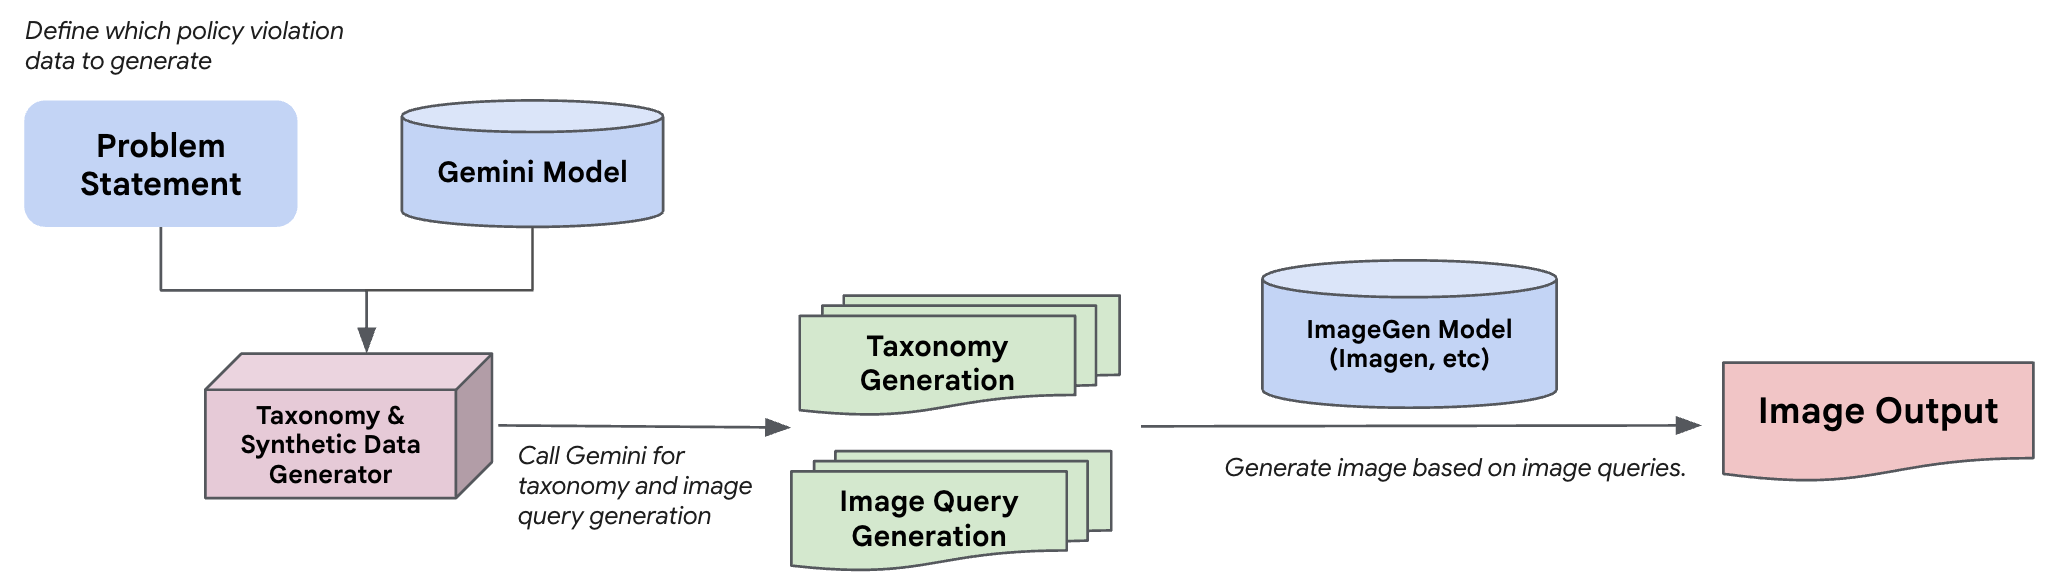
\includegraphics[width=16cm]{figures/data_synth_pipeline.png}
\caption{Synthetic Image Generation Pipeline.}
\label{fig:pipeline}
\end{figure*}

\section{Training Data Curation}
\subsection{Synthetic Data Generation}

The development of SG2 involved a meticulous process of generating synthetic training dataset. This was crucial for creating a robust and comprehensive dataset to train SG2, with the best balance of diversity and severity of images.

Introduced in \cite{davidson2025orchestrating}, our internal data generation pipeline  generates controlled prompts and corresponding images. As illustrated in Fig.\ref{fig:pipeline}, the process includes: 

\begin{itemize}[leftmargin=10pt]
  \item \textbf{Problem Definition}. Encompassing policy definitions, exceptions, input/output formats, and few-shot examples.
  \item \textbf{Taxonomy Generation.} Our Taxonomy \& Synthetic Data Generator produces taxonomy in a one or multi-layer tree structure for each of the dimensions like topics, target demographics (e.g., gender, sexual orientation), the context, regional aspects and image styles (e.g., pixel art, vintage), etc. For example, for the taxonomy of topic, the first layer includes a coarse-grained topics for this harm policy, and the second layer includes additional fine-grained sub-topics.
  \item \textbf{Image Query Generation.} Our generator creates prompts by combining these leaf nodes across all these tree-structured taxonomies. As an example, a dangerous policy with \textit{(Topic=terrorism, sub-topic=arms and ammunition, context=social media, locale=Africa, image style=Pointillism)} could generate: \textsf{Pointillist painting of a man firing an AK-47 into a bustling souk in Marrakech, with market stalls overturned and people scattering in fear.}
  \item \textbf{Image Generation.} We leverage Imagen models \citep{saharia2022photorealistic} to generate around $10k$ images per policy with various aspect ratios and resolutions. The data generation process follows an iterative approach, wherein assessment results informed enhancements, including adjustments to model parameters, refinement of taxonomies, and the incorporation of additional few-shot examples.
\end{itemize}


\subsection{Real Image Selection}

To enhance SG2's performance on real-world images, we leveraged the extensive WebLI (Web Language and Image) dataset \citep{chen2022pali}, a large-scale collection containing approximately 10 billion images and captions:

\begin{itemize}[leftmargin=10pt]
    \item Randomly sampled a substantial subset of images from the WebLI dataset.
    \item Utilized a high-performing text safety classifier to analyze the captions associated with each sampled image.
    \item Retained images where at least one of these categories had a violation probability exceeding 0.1.
    \item From the filtered set of images identified as potentially violating our safety policies, we randomly selected a final training set of $120k$ images.
\end{itemize}

\subsection{Borderline Adversarial Data Generation (BADG)}
Our training labels are generated using in-context learning with the Gemini model (detailed in the section \nameref{sec:labelgen}). To bridge the performance gap between Gemini's in-context learning capabilities and SG2, we generated image prompts which intentionally cause ShieldGemma 1 \citep{zeng2024shieldgemma} to produce misclassifications (both false positives and false negatives) when compared against a much larger auto-rater (i.e. LLM-as-a-judge \citep{gu2024survey}) based on Gemini. By creating a diverse dataset of adversarial images based on these prompts, we specifically designed it to enhance SG2's classification ability for borderline cases.
